\chapter{Problem Presentation}
Given the premises presented in the previous chapters, our work mainly focused on two open issues regarding both the dictionary learning and the graph learning problem. The starting point were the works of Dorina Thanou-  regarding the dictionary learning approach for graph signals - ant the work of Hermina Petric Maretic - regarding the graph learning approach.\\
In the related work, Thanou et al. proposed a learning algorithm which was able to retrieve the kernel functions for a certain dictionary, alternately optimizing over the kernel coefficients $\alpha$ and the sparsity matrix $X$, while Maretic et al. started from the complementary assumption that the entities know in their case where exactly the kernel coefficients, while they alternatively optimized over the sparsity matrix and the graph weight matrix.

\section{State of the art}
There has already been a discrete amount of work around graph inference for signals that are expected to be smooth on the graph.  In \cite{Dong2016} Dong et al. addressed the problem adopting a factor analysis model for graph signals and imposing a Gaussian probabilistic prior on the independent variables which model the signal. Their results showed that smoothness property of a graph signal is favoured by the efficient representation obtained through these priors. In particular, in the algorithm they proposed they deployed the use of $l^1$ and Frobenius norm, the former is expressed by a constraint on the Trace of the Laplacian, and eventually accounts for a sparsity term, while the latter is added as a penalty term in the objective function in order to control the distribution of the off-diagonal entries in L.

At the same time, in \cite{Kalofolias2016} Kalofolias proposes another framework to learn a graph structure under the smoothness assumption. They used as well the minimization of the trace term for the Laplacian matrix, clinching that the minimizations of it brings to naturally sparse solutions.

However, this assumption is not always exhaustively descriptive of the real problem we are considering, so we might want to add other reinforcements to the priors in order to better describe the situation. For example, we could imagine a real world network to show a localized behavior or a more organized one having a certain pattern repeating over the graph. In \cite{Maretic2017}, this was an assumption for the signal, bringing it to be a sparse combination of a small number of atoms in a polynomial graph dictionary. This in the end was creating atoms localized in every node on the graph, repeating the same pattern over it with respect to every node as a source, in the same way it is described in \cite{Thanou2014}. The limitation Thanou's work is mainly the fact that, as we already mentioned, it assumes the kernels to be know function while it concentrates only on the graph dictionary and thus fixing the spectral behaviour of the atoms.

\section{Problem description}
As previously mentioned, this work deals with the general class of signals that can be represented in a sparse way through atoms of a polynomial dictionary \cite{Thanou2014}, such that it can give a natural segregation of each signal into localised components, as shown in \autoref{fig:components}. The figure shows how each of these components derive from one atom directly dependent of the graph dictionary and this is well explained if, for polynomial kernels of degree k, we see our atoms as an entities spanning only the k-hop distance from the node representing the center of the atom (source).

\begin{figure}
\centering
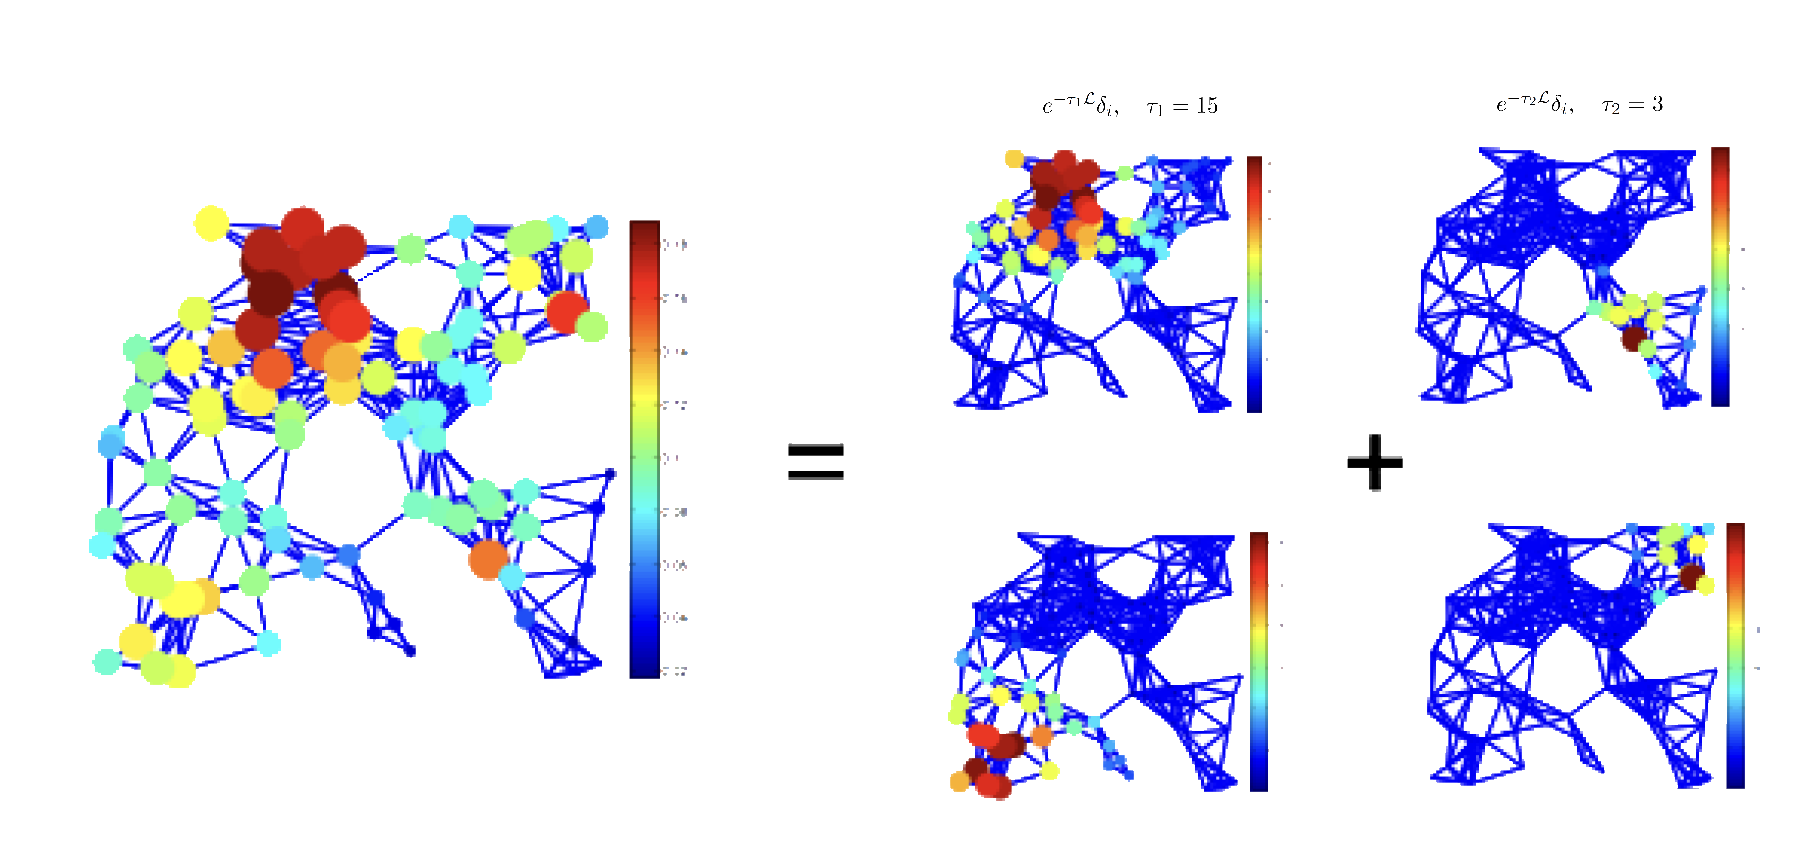
\includegraphics[width = .8\textwidth]{SignalDecomposition.png}
\caption{Example of signal decomposition using the polynomial dictionary}
\label{fig:components}
\end{figure}

\subsection{Assumptions}
\cri{Verifica la faccenda della community structure che stai per scrivere}
In opposition to the prior work, here we assume the sources of our atoms to be known and the same for all signals, meaning that the network has a certain amount of nodes acting like sources an thus controlling the behavior of the network. Another strictly related assumption, is that the graph has a strong community structure, meaning that the graph can be separated into communities which are poorly related among themselves, but hold strong connections inside them. These two assumptions are somewhat exchangeable and the reduction of one of them could be a future interesting aspect to better develop.

\subsection{Representation graph}

\subsection{Dictionary learning section}
If we considered the former formulation for our problem, we would ignore the fact that atoms in $D_{small}$ actually are coming from a graph dictionary, while this is on the contrary something we would like to include in our problem. In fact, we did assume these atoms to be vectors describing the signal, but we kept this part separated from the graph notion. We start from stating that we want that our atoms are representative of the portion of the graph they are covering, and so they should spread with non trivial values over all nodes of the subgraph. This reason mad us constraint our dictionary kernels in a way that they have mostly smooth support in the surroundings of the source node. This information is something different form the smoothness assumption we widely examined in the previous sections, since it adds some information strictly related to the behavior of the kernel itself. In fact, if we learned a smaller order polynomial with constraints in high frequencies, we would not have a large spread of our atoms, things we would like to have since in this way our atoms can represent a large portion of the graph. \cri{rivedila ti prego}

To have this new smoothness constraint, we look at the kernel polynomial:
\begin{equation}
g(\lambda) = \sum_{k=0}^{K}\alpha_k \lambda_k
\end{equation}
and we try to constraint the roots to correspond to the highest eigenvalues. This would change the expression of the kernel and turn our learning problem into a simpler one, since now we are trying to learn a smaller number of coefficients:
\begin{align}
g(\lambda) &= h(\lambda)(\lambda - \lambda_n)(\lambda - \lambda_{n-1})\cdot \dots \cdot (\lambda - \lambda{n-l+1})\\
where \qquad h(\lambda) &= \sum_{k=0}{K-l}\gamma_k\lambda^{k}
\label{eq:polynom}
\end{align}
This formula them can bring to a dictionary problem of this type:
\begin{equation}
\argmin_{\gamma_0,\dots,\gamma_{K-l}X_{small}} ||Y - D_{small}X_{small}||^2_F + \alpha||D_{small}||_1
\label{eq:opt}
\end{equation}
\begin{align}
with \qquad g(\lambda) &= h(\lambda)(\lambda - \lambda_n)(\lambda - \lambda_{n-1})\cdot \dots \cdot (\lambda - \lambda{n-l+1}) \notag\\
h(\lambda) &= \sum_{k=0}{K-l}\gamma_k\lambda^{k} \notag\\
D_i &= [g(L_i)]_{\text{source}_i} \notag\\
0 &\leq g(\lambda) \leq c \label{eq:ProblemPres1}\\
(c-\epsilon)I &\preceq \sum_{s=1}^{S}D_s \preceq (c+\epsilon)I \label{eq:ProblemPres2}
\end{align}
Where the positions of the non-trivial values of $X_{small}$ are known, but the values are to be learned, while the second term in \autoref{eq:opt} accounts for the graph sparsity. Moreover, the last two constraints \ref{eq:ProblemPres1} and \ref{eq:ProblemPres2} are taken from \cite{Thanou2014} and ensure the kernels are bounded and span the entire spectrum.
\label{sec:DictionaryLearningSection}

\subsection{Joint large graph and dictionary learning}
So came to this point, an interesting aspect we could focus on was the attempt to joint both the graph and the dictionary learning problem; in fact, if we assume that the graph is unknown we could imagine adding a graph learning part to the optimization. In doing this, we had to take into account two main complications: first the fact that we didn't have fixed eigenvalues, since we would have learned the Laplacian again at every new optimization step, and second the fact that as we are learning the eigenvalues, we don't have their initial values either. To this aspects we still have to take into account that the structure of the kernels should be incorporated in our learning problem. For this part, in the end we assumed only one kernel for simplicity so that the dictionary atoms will have all the same kernel but will be localized in different sources spreading throughout different parts of the graph. This meaning that the pattern has to be followed by all the atoms, but it will be adapted to small different graphs.

Therefore the overall problem could become something similar to:
\begin{equation}
\argmin_{X,W_1,\dots,W_m,\gamma_0,\dots,\gamma_{k-l}} ||Y - DX||^2_F + \alpha||D||_1
\label{eq:overallProblem}
\end{equation}
\begin{align}
\text{where} \qquad g(\lambda) &= h(\lambda)(\lambda - \lambda_n)(\lambda - \lambda_{n-1})\cdot \dots \cdot (\lambda - \lambda{n-l+1}) \notag\\
h(\lambda) &= \sum_{k=0}{K-l}\gamma_k\lambda^{k} \notag\\
D_i &= [g(L_i)]_{\text{source}_i} \notag\\
L_i &= \text{normalised Laplacian}(W_i) \notag\\
W_{ij} &= W_{ji} \geq 0, \quad \forall i,j \label{eq:symmetry}\\
W_{ii} &= 0, \quad \forall i \notag\\
0 &\leq g(\lambda) \leq c \\
(c-\epsilon)I &\preceq \sum_{s=1}^{S}D_s \preceq (c+\epsilon)I
\end{align}
Where we remember the constraint in \ref{eq:symmetry} accounts for the fact that we are assuming to work with undirected graphs.\\

\subsection{Work structure}
To summarize, the main steps in which the following work is articulated are the following:
\begin{itemize}
\item We implemented some constraints related to the smoothness of the kernels in the dictionary learning approach, and we showed the improvements deriving from it;
\item We presented a solution to solve both the dictionary and the graph learning problem within the same framework;
\item We underlined how the smoothness constraints on the kernels can still provide improvements even in the case of double learning frameworks;
\item We briefly present the possible next steps in this work, in order to obtain further implementations;
\end{itemize}
